\part{The build process}
\frame{\partpage}

\begin{frame}{Executing programs}
    \begin{itemize}
        \item CPUs execute \textbf{machine code}
        \item Programs must be \textbf{translated} into machine code for execution
        \item There are three main ways of doing this:
        \begin{itemize}
            \item An \textbf{interpreter} is an application which reads the program source code and executes it directly
            \item A \textbf{compiler} is an application which converts the program source code into executable machine code
            \item A \textbf{just-in-time (JIT) compiler} is halfway between the two --- it compiles the program on-the-fly
                at runtime
        \end{itemize}
    \end{itemize}
\end{frame}

\begin{frame}{Examples}
	\begin{columns}[t,onlytextwidth]
		\begin{column}{0.3\textwidth}
		    Interpreted:
		    \begin{itemize}
		        \item Python
		        \item Lua
		        \item Bespoke scripting languages
		    \end{itemize}
		\end{column}
		\begin{column}{0.3\textwidth}
		    Compiled:
		    \begin{itemize}
		        \item C
		        \item C++
		        \item Swift
		    \end{itemize}
		\end{column}
		\begin{column}{0.3\textwidth}
		    JIT compiled:
		    \begin{itemize}
		        \item Java
		        \item C\#
		        \item JavaScript (in modern web browsers)
		        \item Jython
		    \end{itemize}
		\end{column}
	\end{columns}
\end{frame}

\begin{frame}{Interpreter vs compiler}
    \begin{itemize}
        \item Run-time efficiency: compiler $>$ interpreter
        \begin{itemize}
            \item The compiler translates the program \textbf{in advance}, on the developer's machine
            \item The interpreter translates the program \textbf{at runtime}, on the user's machine
        \end{itemize}
        \item Portability: compiler $<$ interpreter
        \begin{itemize}
            \item A compiled program can only run on the operating system and CPU architecture it was compiled for
            \item An interpreted program can run on any machine, as long as a suitable interpreter is available
        \end{itemize}
        \item For games, run-time efficiency is usually much more important than portability
    \end{itemize}
\end{frame}

\begin{frame}[fragile]{The C++ build process}
    \textbf{Preprocessor}
    \begin{itemize}
        \item Replaces \lstinline{#include} directives with the contents of the appropriate header files
        \item Handles other preprocessor directives (\lstinline{#define}, \lstinline{#if} etc --- more on these another time)
    \end{itemize}
    \textbf{Compiler}
    \begin{itemize}
        \item Translates each source file into an \textbf{object file} containing machine code
    \end{itemize}
    \textbf{Linker}
    \begin{itemize}
        \item Combines the object files together with any external libraries to produce an \textbf{executable}
            (on Windows, a .exe file)
    \end{itemize}
\end{frame}

\begin{frame}[fragile]{The C++ build process}
    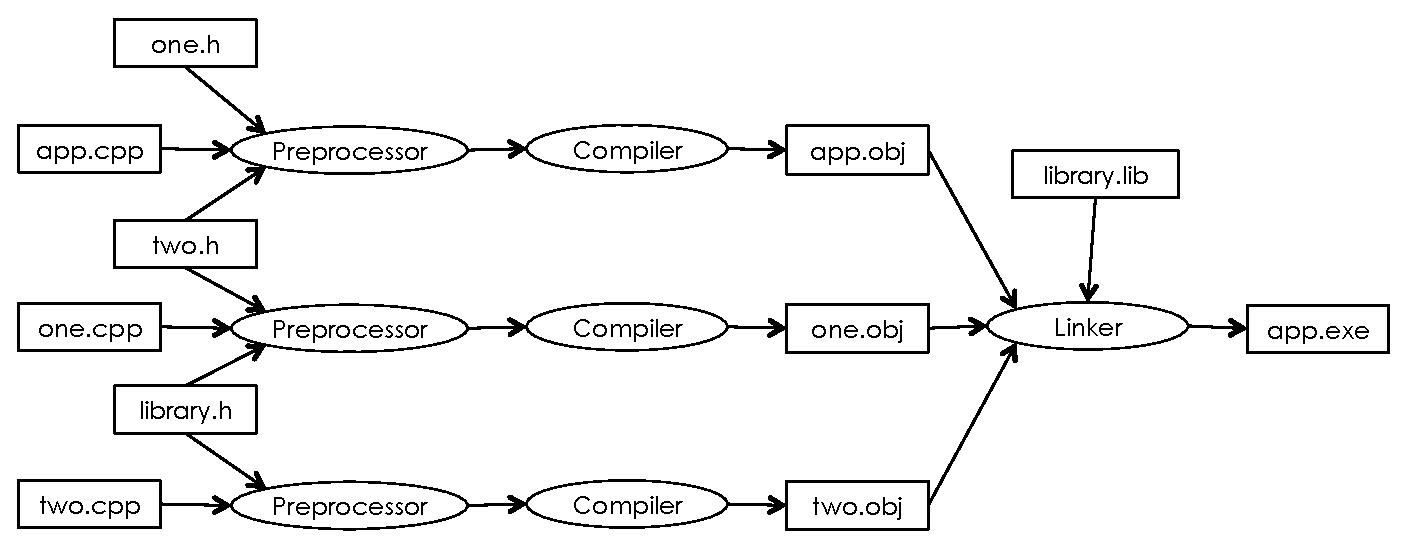
\includegraphics[width=\textwidth]{compiler_flowchart.pdf}
\end{frame}

\begin{frame}[fragile]{Incremental compilation}
    \begin{itemize}
        \item Compilation takes time --- compiling a AAA game can take several hours
        \item Visual C++ stores intermediate files (e.g.\ \texttt{.obj} files) on disk
        \item Only the changed files need to be run through the preprocessor and compiler again
            $\implies$ faster re-compilation during development
        \item \textbf{Build $\to$ Clean} removes all intermediate files
        \item \textbf{Build $\to$ Rebuild} forces Visual C++ to recompile everything
    \end{itemize}
\end{frame}

\begin{frame}[fragile]{Precompiled headers}
    \begin{itemize}
        \item Headers may need to be compiled multiple times if they are included in multiple source files
        \item Headers may be very large ---
            e.g.\ \texttt{Windows.h} includes dozens of headers totalling many thousands of lines
        \item In Visual C++ projects, \texttt{stdafx.h} is a \textbf{precompiled header}
        \item \lstinline{#include "stdafx.h"} doesn't work like copy and paste ---
            instead, the compiler uses the precompiled header information
        \item Precompiled header only needs to be recompiled if \texttt{stdafx.h} (or something it includes)
            changes, which should be rare
    \end{itemize}
\end{frame}

\begin{frame}[fragile]{Build configuration in VC++}
    \begin{center}
        
\includegraphics[width=0.6\textwidth]{vcpp_build_toolbar.PNG}
    \end{center}
    \begin{itemize}
        \item Configuration:
        \begin{itemize}
            \item \textbf{Debug} allows use of the Visual C++ debugger
            \item \textbf{Release} produces optimised code --- usually 2--10 $\times$ faster than Debug
            \item Generally use Debug for development, Release for optimisation and distributing the finished application
        \end{itemize}
        \item Platform:
        \begin{itemize}
            \item \textbf{x86} runs on 32-bit and 64-bit versions of Windows
            \item \textbf{x64} runs on 64-bit Windows only
            \item Generally use x86 for maximum compatibility, x64 for apps which need to use $>2$GB memory
                or where a significant speed benefit is measured
        \end{itemize}
    \end{itemize}
\end{frame}
